\documentclass{article}
%\documentclass{scrartcl}

\usepackage {amsmath}
\usepackage {textcomp}
\usepackage {setspace}
\usepackage [pdftex]{graphicx}
\usepackage[sort&compress]{achemso}
%\usepackage{lineno}

% For typesetting roman numerals
\makeatletter
\newcommand{\rmnum}[1]{\romannumeral #1}
\newcommand{\Rmnum}[1]{\expandafter\@slowromancap\romannumeral #1@}
\makeatother

% some formatting tags
\usepackage[
top    = 0.5in,
bottom = 1.5in,
left   = 2.50cm,
right  = 2.50cm]{geometry}
%\oddsidemargin  0.0in
%\evensidemargin 0.0in
%\topmargin -0.5in
%\bottommargin -0.5in
%\textwidth      6.5in

\title{Bonding, Intimacy, and Circles of Friends: Further Computational Studies of Sulfur Dioxide Adsorption to Aqueous Surfaces}
\author{Eric S. Shamay \and Geraldine L. Richmond}

\begin{document}

\newcommand{\suldiox}{SO$_2$}
\newcommand{\ang}{\,$\textrm{\AA}$}
\newcommand{\angs}{\ang}
\newcommand{\wat}{H$_2$O}

\maketitle

%\onehalfspacing
%\linenumbers 
\doublespacing


\begin{abstract}
A water surface is a dynamic and constantly evolving terrain producing a vast array of unique molecular properties and interactions with environmental chemical species. The dynamics of water surfaces permit life on earth to continue, but also keeps us from developing a complete microscopic picture of the specific behaviors that take place within interfacial aqueous environments. This computational study examines a piece of the water puzzle by elucidating the bonding, dynamic interactions, and hydrate structures of sulfur dioxide gas adsorbing to a water surface. Results described herein address the specific ways in which sulfur dioxide gas molecules bind to a water surface, and paint a more complete picture of the adsorption pathway than was previously developed from experimental and computational studies. Ab initio molecular dynamics have been employed to study sulfur dioxide and water interactions at two environmentally relevant temperatures on a water surface. The results of this study on a common environmental and industrially important gas provide molecular insight to aid our understanding of interactions on aqueous surfaces, and gaseous adsorption processes.
\end{abstract}

\section {Introduction}

One of chemistry's many remaining ``black box'' events is the adsorption of a gas into a water surface. Although gas uptake into aqueous systems occurs often environmentally and industrially, we still know very little about the process and the details of the adsorption reactions. How does gas bind to a water surface, and what steps are involved in adsorption? How does a gas molecule near a water surface affect the water to which it will bind? What is the structure of hydrating waters in the surface region, and how does that hydrated solute molecule behave differently than as a gas? Experiments to address these questions provide valuable information, but can never fully describe these microscopic events and behaviors. The information can be determined computationally, and when coupled to the previous experimental work can provide a much more complete picture of gaseous adsorption to aqueous surfaces.

As a model gas, \suldiox~has been used extensively in research because of its importance in commercial and environmental systems. The molecular structure, high solubility in water, and its abundance make it a pivotal compound in numerous aqueous atmospheric reactions. A complete picture of the \suldiox~adsorption process will aide in understanding gaseous adsorption on the many aqueous surfaces in the environment, as well as in understanding the fundamental nature of gases in water interfacial regions. 

In this study we use ab initio quantum molecular dynamics (MD) techniques to model and simulate the hydrating structure that forms around a surface-bound \suldiox~on water. We simulate a dynamic water surface with an extended hydrogen-bonding network that captures the fluidity of the \suldiox~hydrate structures, and the behaviors on the water surface. Unlike small cluster studies that use DFT calculations on geometry optimized structures to find likely geometries in a static vacuum setting, The quantum MD technique allows us to simulate the process much more realistically, and with greater accuracy than our previous classical MD work could allow.\cite{Shamay2011} This computational study greatly enhances the picture developed in our previous work on \suldiox. In our previous computational study we used classical MD to determine net orientational behavior of \suldiox~binding to a water surface, and of the orientation of the waters in response to the presence of an adsorbing gas. Understanding the net behavior of the molecules in the aqueous interfacial region throughout adsorption was the first step to understanding the specific details of gas binding and surface behavior. 

Quantum MD techniques accurately reproduce the hydration geometry around the bound \suldiox~molecules, and allow us to look at the specific bonding interactions that form within the surface hydrates, and in the extended bonding further into the water. The surfaces in this work were simulated at two temperatures: room temperature at 298K, and the more atmospherically relevant cold 270K. This set of temperatures complements our most recent experimental studies that showed the binding of gaseous \suldiox~to a water surface is greatly enhanced at cold temperatures.\cite{Ota2011} Other experiments by our group developed the picture of \suldiox~adsorption, and showed that \suldiox~surface hydrate complexes form when a water surface is exposed to \suldiox~gas.\cite{Tarbuck2005,Tarbuck2006} Conclusions from the experiments regarding the specific nature of those complexes could only be inferred. 

We believe this to be the first temperature study using quantum MD to look at the binding of a small gas molecule to a water surface. We show how temperature affects the bonding behavior of the surface adsorbed \suldiox~to neighboring waters. A proposed set of steps in a binding mechanism for \suldiox~adsorbing to a water surface is presented. We also look at \suldiox~behavior when already bound by the surface waters. Lastly, our analysis shows some interesting extended bonding behavior of \suldiox~hydrates, and that the hydrating waters and the \suldiox~often form cyclic ring structures through intermolecular bonds.

\section {Background}

\subsection {Bonding Coordination}

A hydrated \suldiox~in an aqueous environment forms hydrogen bonds through the oxygens to nearby water-hydrogens, or interacts via the sulfur atom with water-oxygens. To further our analysis of the way in which \suldiox~coordinates its bonding to surface waters (those that lie in the topmost region of a gas/water interface), we adopt a naming scheme to denote the way in which the \suldiox~is hydrated by the surrounding waters. This naming scheme mimics a notational system developed during a previous study on water coordination by Buch et al,\cite{Buch 2005} and was subsequently used in more recent computational work.\cite{Walker2006b} In this naming system, a letter is used to designate the atom on a water molecule through which a hydrogen bond is formed to neighboring waters. Thus a bonding coordination of ``OOH'' designates two proton-acceptor bonding interactions through the water-oxygen, and a single proton-donor bonding interaction through a hydrogen. More recently, Baer et al. devised a nomenclature that explicitly enumerates the bonding to \suldiox~via the sulfur or oxygen atoms.\cite{Baer2010} 

In this work we adopt a nomenclature scheme for \suldiox~in order to quantify hydrogen bonding through the acceptor \suldiox-oxygens, and the weaker bonding interactions from the \suldiox-sulfur to water-oxygens. Thus, an ``SOO'' coordinated \suldiox~molecule forms a single interaction through the sulfur atom to a neighboring water-oxygen, and two hydrogen bonds through either a single \suldiox-oxygen, or distributed with one hydrogen bond on each of the \suldiox-oxygens. Analysis of the distribution of \suldiox~coordinations will give insight to how \suldiox~binds to the water surface.

To determine \suldiox~bonding coordinations, we defined intermolecular bonds using the distance criteria of Baer et al.\cite{Baer2010} The bond-length definition is based on a set of distance criteria where a bonding interaction between a \wat-oxygen and \suldiox-sulfur is formed at a distance less than 3.5 \angs, and an \suldiox-oxygen hydrogen bond to a \wat-hydrogen is formed at a distance less than 2.2 \angs.

\subsection {Cyclic Bonding Structures}

Hydrated \suldiox~clusters have been studied extensively with many recent experiments and computations forming a clearer picture of \suldiox~bulk and surface behaviors.\cite{Baer2010, Tarbuck2005, Tarbuck2006, Ota2011, Bishenden1998, Hirabayashi2006, Steudel2009, Yang2002, Hayashi1985, Moin2011, Eckl2008} At a water surface, it is now known that \suldiox~forms a complex with water during adsorption, and then subsequently absorbs into the interfacial region by reaction to form ionic sulfur species.\cite{Tarbuck2005, Tarbuck2006, Ota2011} The first attempt to elucidate the structure of surface hydrated \suldiox~by Baer et al. showed that the bonding coordination distributions of \suldiox~are altered relative to the bulk region, and that two coordinations dominate the distribution of bonding types: the ``SO'' and the ``SOO''. In the same work they then focused on the dominant coordination to determine the most likely cluster geometry using two and three-water clusters bound to the \suldiox. However, none of the studies have yet focused directly on the presence of an extended hydrating structure involving closed rings of molecular interactions involving the solvated \suldiox~molecules.

The cluster geometries found in this study imply a cyclic bonding structure through the two or three waters involved. ``Cyclic'' here is used to denote a closed loop formed by the intermolecular hydrogen bonds, S-O interactions, and covalent bonds of the molecules involved. Figure \ref{fig:cyclic-example} depicts one such cyclic structure showing the bonds beginning on the sulfur and returning through a \suldiox-oxygen.

\begin{figure}[h!]
	\begin{center}
		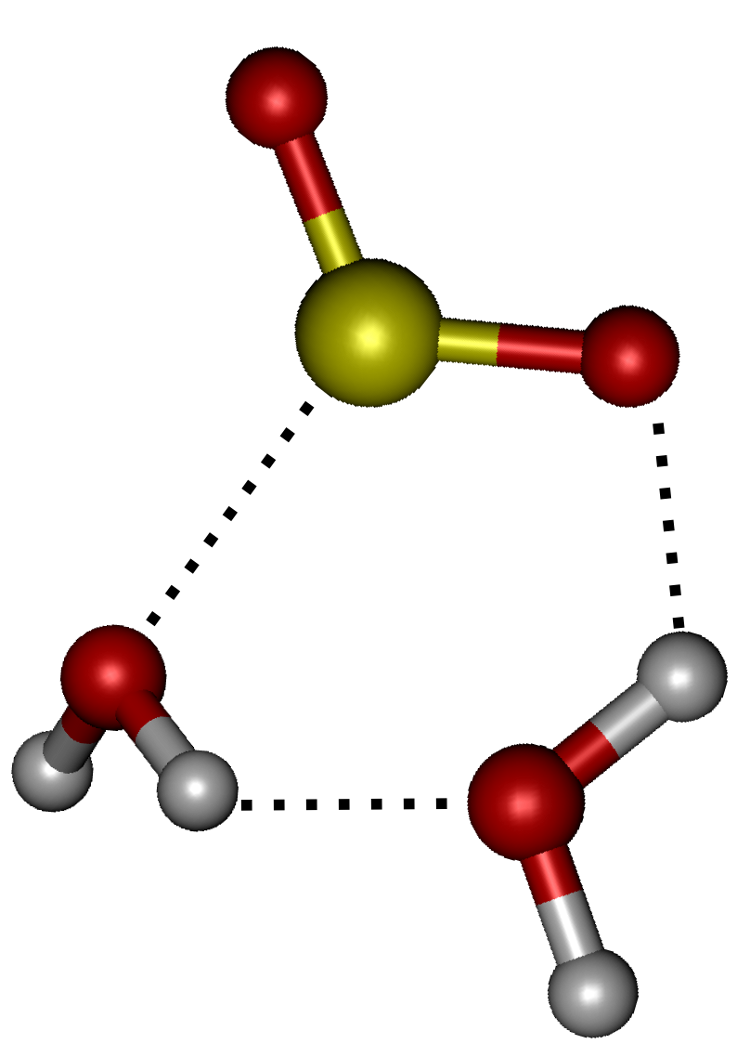
\includegraphics[scale=1.0]{images/cycles/double-cycle-type2-small.png}
		\caption{During the course of MD, the covalent and intermolecular bonds between a \suldiox~and the hydrating waters may form into a ring, resulting in a cyclic hydrate structure. Depicted here is one example of such a cyclic structure, formed by the covalent SO and OH bonds of the two molecule types, and the intermolecular hydrogen bonds, and S-O$_{H_2O}$ interactions. The atoms involved are the S (yellow), O (red), and H (white).}
		\label{fig:cyclic-example}
	\end{center}
\end{figure}

\subsection {Graph Theoretical Details}
The optimized geometry of the \suldiox-hydrates suggests cyclic bonding structures, but it remains a different story entirely when \suldiox~is placed in a dynamic environment such as in the course of MD simulations of an aqueous surface. Geometry optimization shows the formation of these cyclic hydrate structures with two or three waters in a static vacuum. Do the cyclic structures also form in the course of a dynamic bonding process on a simulated water surface, where extended hydrating structures influence \suldiox~and water behavior? To study the formation and behavior of cyclic hydrate structures we employ graph theoretical techniques on MD trajectory data. Previous use of graphs in molecular computations were applied to finding stable arrangements of water clusters, ice, hydrogen bonding, extracting topological molecular properties, and cyclic structure studies.\cite{Anick2002, Huber2007, Radhakrishnan1991, Shi2005, Garcia2004, McDonald1998}

Here we briefly introduce graph theoretical concepts. They have been described well by others with varied application to cyclic structures.\cite{Tutte1984, Balakrishnan2000, Harary1973, Huber2007, Garcia2004, Dury2001} A graph consists of nodes, and edges that connect the nodes. A molecule can be represented with atoms as nodes, and edges for each intramolecular covalent bond connecting the atoms. The set of edges is then further expanded to include intermolecular interactions such as hydrogen bonds and other bonding interactions. Edges may be assigned weights (i.e. bond lengths), types, and can be directional, i.e. pointing towards a target node from a source node. A molecular system including all atoms, bonds, and interactions is thus fully described by a graph. 

To detect cyclic structures in a graph a depth-first or breadth-first search (DFS and BFS, respectively) may be used.\cite{Knuth1997, Cormen 2001} A BFS is a recursive algorithm of queuing nodes and all neighboring nodes while performing a specified procedure on each visited node. This is easily performed on adjacency list or connectivity matrix data structures, iterating through nodes (i.e. atoms) of interest in the graph as starting points of the search. In BFS terminology, all nodes are colored during graph traversal to distinguish unvisited nodes (white), queued nodes (gray), and visited nodes (black). Using a BFS on a graph, cyclic structures are detected any time a ``gray target'' is encountered when queuing adjacent neighbors of a node. A benefit of BFS on a graph is the ability to determine the smallest cyclic structure containing a given node. In the case of \suldiox~hydrate structures, beginning the BFS with the \suldiox-sulfur as the starting, or root node for the search, will discover cyclic bonding structures in order of size. Here we are only concerned with the smallest cyclic structure involving those waters in the first and second hydration shells around the \suldiox. Furthermore, it is possible to reconstruct a cycle's structure by finding its size (number of contributing atoms), and the number of unique waters in the cycle. This allows us to distinguish between various types of cyclic structures encountered.

Several arrangements of cyclic bonding structures are shown in Figure \ref{fig:cyclic-structures} for a \suldiox~molecule with three waters. Cycles with fewer or greater numbers of waters are also possible and encountered during MD. Cycle types \Rmnum{1}, \Rmnum{2}, \Rmnum{3} in Figure \ref{fig:cyclic-structures} are cyclic structures in which the \suldiox~is a member of the cycle. Types \Rmnum{4} and \Rmnum{5} do not involve the \suldiox~in the bonding cycle, but are commonly encountered as the smallest cycle types formed near the \suldiox. Type \Rmnum{3} is of particular interest because the \suldiox~in this cycle has the most frequently occuring bonding coordination (``SO'', as shown later).

\begin{figure}[h!]
	\begin{center}
		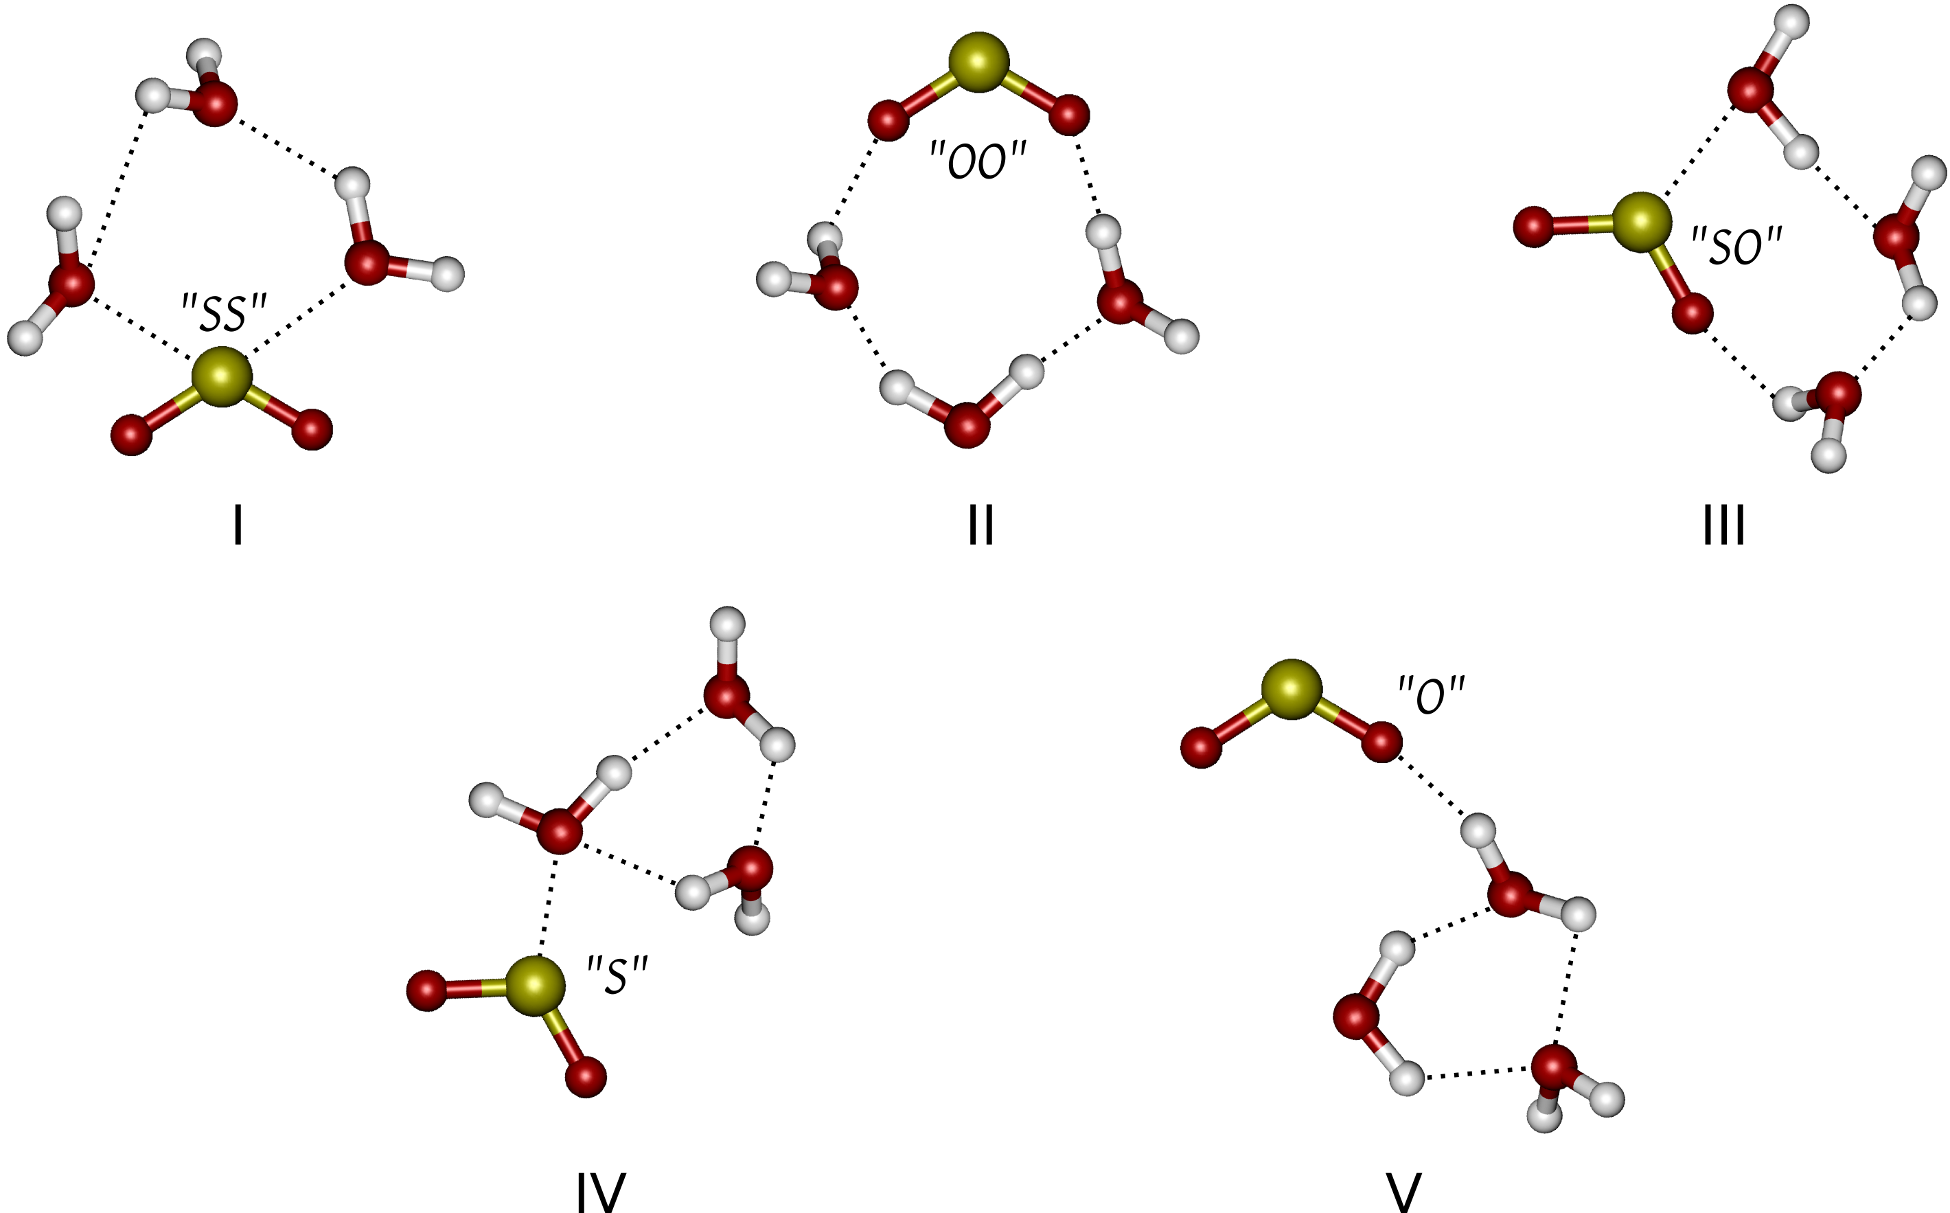
\includegraphics[scale=1.0]{images/cycles/cycle-types-small.png}
		\caption{\suldiox~in various cyclic structures encountered during MD simulations with water. The cartoons show the five types of cyclic structures, numbered for reference. The cyclic structures may involve any number of waters, but here each structure is shown with three waters. Type \Rmnum{3} is formed by a \suldiox~with the ``SO'' bonding coordination, which is the most dominant bonding coordination encountered.}
		\label{fig:cyclic-structures}
	\end{center}
\end{figure}

Baer et al. presented a detailed geometric and spectroscopic breakdown of type \Rmnum{3} cycles with two and three waters from their DFT calculations.\cite{Baer2010} Given the information of the number of waters, atoms, and bonds involved in the bonding cycles, we find that of the three-water type \Rmnum{3} cycles, there exist two structural varieties, shown in Figure \ref{fig:type-3-varieties}, that differ in the set of water atoms involved in the cyclic structure. Type \Rmnum{3}-A (shown in Figure \ref{fig:type-3-varieties}A) is arranged with each water contributing an OH bond to the structure of the cycle. Type \Rmnum{3}-B involves a single water contributing an OH, whereas the other two waters contribute only the oxygen atom or the entire water molecule to the structure, respectively. This nuance of the type \Rmnum{3} structures involving three waters, and the overall distribution are presented in more detail later. We also show the distribution of cyclic structures encountered during MD simulations to further understand the behaviors of \suldiox-hydrates at the water surface.

\begin{figure}[h!]
	\begin{center}
		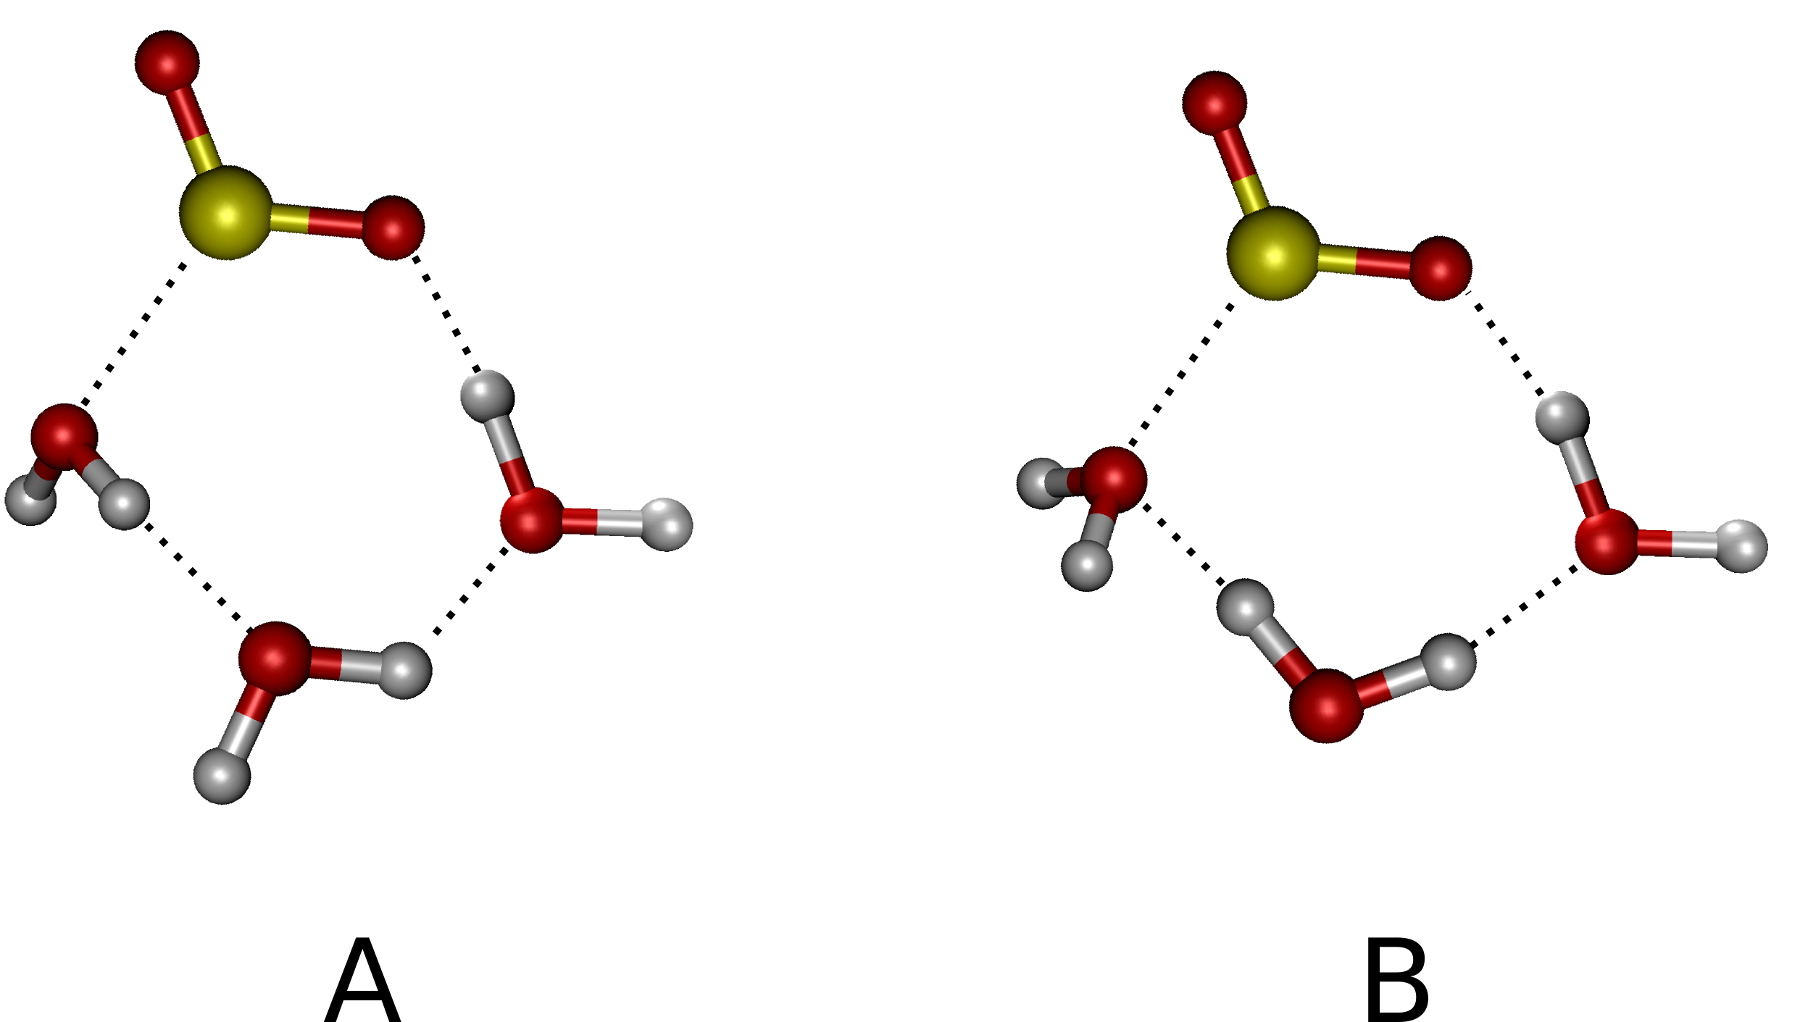
\includegraphics[scale=1.0]{images/cycles/triple-cycle-types-small.png}
		\caption{Type \Rmnum{3} cyclic structures (see Figure \ref{fig:cyclic-structures}) are found to occur in two varieties that are distinguished by the water atoms contributing to the cyclic structure. In ``type A'' the cycle is formed by an OH bond contributed by each water, and the SO bond of the \suldiox. ``type B'' involves an oxygen atom from one water, an OH bond from a second water, and all atoms of the third water.}
		\label{fig:type-3-varieties}
	\end{center}
\end{figure}

\section{Computational Methods}

On-the-fly ab initio molecular dynamics simulations were performed with the QUICKSTEP package, which is an implementation of the Gaussian plane wave method using the Kohn-Sham formulation of density functional theory (DFT).\cite{VandeVondele2005} The Kohn-Sham orbitals are expanded using a linear combination of atom-centered Gaussian-type orbital functions. The electronic charge density was described using an auxiliary basis set of plane waves. Energies and forces from on-the-fly simulation sampling of the Born-Oppenheimer surface were calculated for each MD step using the Gaussian DZVP basis set, the exchange-correlation functional of Becke, Lee, Yang, and Parr (BLYP),\cite{LEE1988} and the atomic pseudo-potentials of the Goedecker, Teter, and Hutter type.\cite{Goedecker1996} A simulation timestep of 1 fs was used, with a Nose-Hoover thermostat set at 273K and 300K for the ``cold'' and ``hot'' simulations, respectively. These computational parameters were verified to yield a reasonable description of bulk room temperature water when simulating a neat-water system. 

Initially, 10 equilibrated boxes of side-lengths 10.0\angs, with 36 randomly packed water molecules were used. Five of the boxes were used for each of the cold and hot simulations. A sulfur dioxide molecule was randomly placed onto the surface within 2.5\angs~of a water molecule centrally located above the waters in the z-axis. A copy of the initial system cubes were then expanded along one axis (z-axis) to 25\angs. The system energy was minimized through a geometry optimization. Subsequently, the system was equilibrated for 1 ns in canonical ensemble (NVT) conditions. Periodic boundaries were set on the two short axes to form an infinite slab. The equilibrated systems were then simulated for a further 20 ps in the microcanonical ensemble (NVE), with trajectory snapshots recorded every 1 fs. The initial 1 ns equilibration trajectory was not included in the final analysis. This simulation process resulted in 20,000 time steps of system trajectory for analysis in each of the hot and cold replicas of the system, for a total of 100,000 timesteps at each temperature.
 

\section {Sulfur Dioxide Bonding Coordinations}

The bonding coordination of each \suldiox~was determined at each timestep of the simulations. Figure \ref{fig:bonding-coordinations} shows the distribution of bonding coordinations of the surface \suldiox, as a percentage of all bonding coordinations encountered for both the cold (blue) and hot (red) trajectories. A first visual inspection reveals several trends. Clearly the ``SO'' coordination is the most populous at both temperatures. The second and third most populated coordinations are the ``S'' and ``SOO'', however their distributions differ between temperatures. In cold simulations the ``S'' and ``SOO'' coordinations occur nearly equally. The hotter temperature simulation shifts the distribution such that the ``S'' occurs 5\% less frequently than in the cold, and the ``SOO'' occurs nearly 10\% more often. The distribution of bonding coordinations in the hot temperature has a clear first and second most frequent coordination: ``SO'' and ``SOO'', respectively. These results for the hot (room temperature) system coincide with those of the previous single-temperature simulation study by Baer et al. at a similar temperature.\cite{Baer2010}

\begin{figure}[h!]
	\begin{center}
		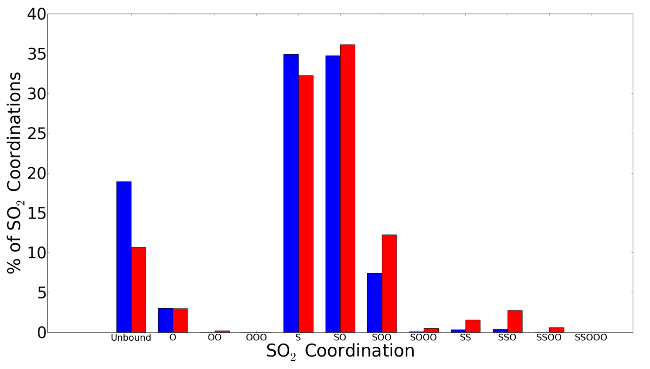
\includegraphics[scale=1.0]{images/coordinations/so2-coordinations-percents-small.png}
		\caption{The \suldiox~bonding coordinations occur with different frequencies at the surface under hot and cold temperature conditions. Shown above is the distribution of bonding coordinations of the cold (blue) and hot (red) \suldiox~over the entire set of trajectories. The values are the percentage of MD timesteps spent in the given bonding coordination.}
		\label{fig:bonding-coordinations}
	\end{center}
\end{figure}

	Several conclusions about the bonding behavior of \suldiox~to surface waters stem from this distribution of coordinations. Clearly the cold \suldiox~spends more time than the hot \suldiox, 13\% versus 3\%, respectively, completely unbound from the surface waters. This does not necessarily imply a complete desorption into the gas phase, but only a brief sojourn away from the waters, with all interactions and bond lengths longer than the cutoff criteria used for the analysis. Furthermore, the most frequently occurring bonding coordinations are ``S'',``SO'', and ``SOO'', with ``SO'' being the most populated at both temperatures. Baer et al. also concluded that these three coordinations were the most frequent for a room temperature simulation, and specifically identified the ``SO'' and ``SOO'' as most common in their study.\cite{Baer2010}

	Looking closer at the coordination types it is notable that coordinations lacking any sulfur interactions (e.g. ``O'', ``OO'', etc.) represent the least frequently formed. A bonding coordination with at least a single sulfur interaction is clearly favored over \suldiox~``oxygen-only'' bonding to waters. In our previous classical simulations of \suldiox~on water we concluded that during adsorption and throughout the interface, the \suldiox~orients so that its sulfur tends to the \wat~bulk side of the interface.\cite{Shamay2011} The coordination distributions here support the idea that binding through the sulfur is preferable, to the extent that a non-sulfur coordination is rarely formed during the course of all our simulations.

% Baer's assymetric oxygen binding
Baer et al performed this coordination analysis for their single-temperature study, but discriminated between \suldiox~binding through the two different oxygens. They concluded that there is asymmetric hydrogen bonding through the \suldiox-oxygens, with one oxygen binding more often than the other. This is supported by the findings here where all the double oxygen coordinations (e.g. ``OO'', ``SOO'', etc.) represent a much lower percentage of the coordinations than the single oxygen counterparts (e.g. ``O'', ``SO'', etc.). Furthermore, a triple-oxygen coordination (e.g. ``OOO'', ``SOOO'', etc.) is very rarely encountered. Three \suldiox-oxygen bonds only form if both \suldiox-oxygens are interacting with water hydrogens. Our finding that triple-oxygen coordinations rarely form complements Baer et al's conclusion about the asymmetry in the oxygen interactions.

Having established the preference for an interaction through the \suldiox-sulfur atom, we look to the right side of Figure \ref{fig:bonding-coordinations} at the double-sulfur coordinations (e.g. ``SS'', ``SSO'', ``SSOO'', etc.). We see from the data that single-sulfur coordinations are overwhelmingly preferred over double-sulfur ones. Adding a third oxygen atom is also unfavorable as the ``OOO'' and ``SSOOO'' together represent less than 1\% of the trajectories, and the comparison between ``SOO'' to ``SOOO'' shows a very large decrease in occurrences.

We can now form a picture of a typical \suldiox~molecule adsorbed to a water surface across both temperatures in this study. The \suldiox~will have at least one interaction to neighboring waters through the sulfur, and will then bond asymmetrically through one of the oxygens either once or twice to water hydrogens. The \suldiox-oxygen bonds will form and break repeatedly throughout a trajectory, and overall the most dominant coordination will be the ``SO'' bonding arrangement.


\subsection {Temperature Effects on Bonding Coordinations}

The binding behavior of the \suldiox~is altered by changing the temperature of the system, as evidenced in the shift in bonding coordination populations of Figure \ref{fig:bonding-coordinations} from cold to hot. In the cold temperature, the unbound, ``S'', and ``SO'' coordinations are more populated than in the hot systems. The increased temperature decreases the time spent in the unbound coordination, and causes all the coordinations to the right of ``SO'' in Figure \ref{fig:bonding-coordinations} to increase over the equivalent cold temperature populations. We see that the cold \suldiox~spends nearly four times as much time unbound as the hot \suldiox, with most of the unbound population in the hot simulations shifting to coordinations with double-oxygen and double-sulfur bonds. 

On the cold water surface, the ``S'' and ``SO'' are more populated than for the hot system. The relative decrease of these coordinations are matched in the hot surface by an increase of the ``SOO'' configuration. This speaks to a dramatic difference in the surface behavior of \suldiox~at the two temperatures. The cold \suldiox~spends nearly equal time in the ``S'' and ``SOO'' coordinations, but nearly 20\% more time in the ``SO''. Thus, the addition or removal of a bond through the \suldiox-oxygen to a neighboring coordination (e.g. addition of an oxygen bond from ``SO'' to ``SOO'', or removal of the bond from ``SO'' to ``S'') is equally probable, as long as the sulfur interaction with the water oxygen does not break. 

Figure \ref{fig:rdf} shows the radial distribution functions (RDF) of \suldiox~to water atoms for both cold (blue) and hot (red) temperatures. The S-O$_{H_2O}$ RDFs are nearly equal except for a slightly taller first peak in the cold system. Along with the slightly larger population of the cold ``S'' and ``SO'' coordinations in the cold surface, the RDF indicates that since bonding occurs frequently through the sulfur, the cold \suldiox-sulfur interacts more closely with the surface waters. In the hot systems, the bonding coordinations with two oxygen bonds (e.g. ``SOO'', etc.) occur more frequently than in the cold system. This additional bonding through a second oxygen interaction may slightly shift neighboring hydrating waters away from the \suldiox-sulfur towards the oxygen end of the molecule. This suggests that the cold \suldiox~bonds closer to the surface waters through its sulfur atom (as shown in the S-O$_{H_2O}$ RDF) and favors the more ``sulfur-centric'' bonding coordinations (e.g. ``S'', ``SO''). The increased temperature of the hot system allows the \suldiox~to bond more extensively through its oxygens to the ``SOO'' coordination. The greater interactions through the oxygens, and higher bonding coordination, may pull the \suldiox~further into the water interface and then allow for increased bonding through the sulfur, up to double-sulfur coordinations (e.g. ``SS'', ``SSO'', etc.).

\begin{figure}[h!]
	\begin{center}
		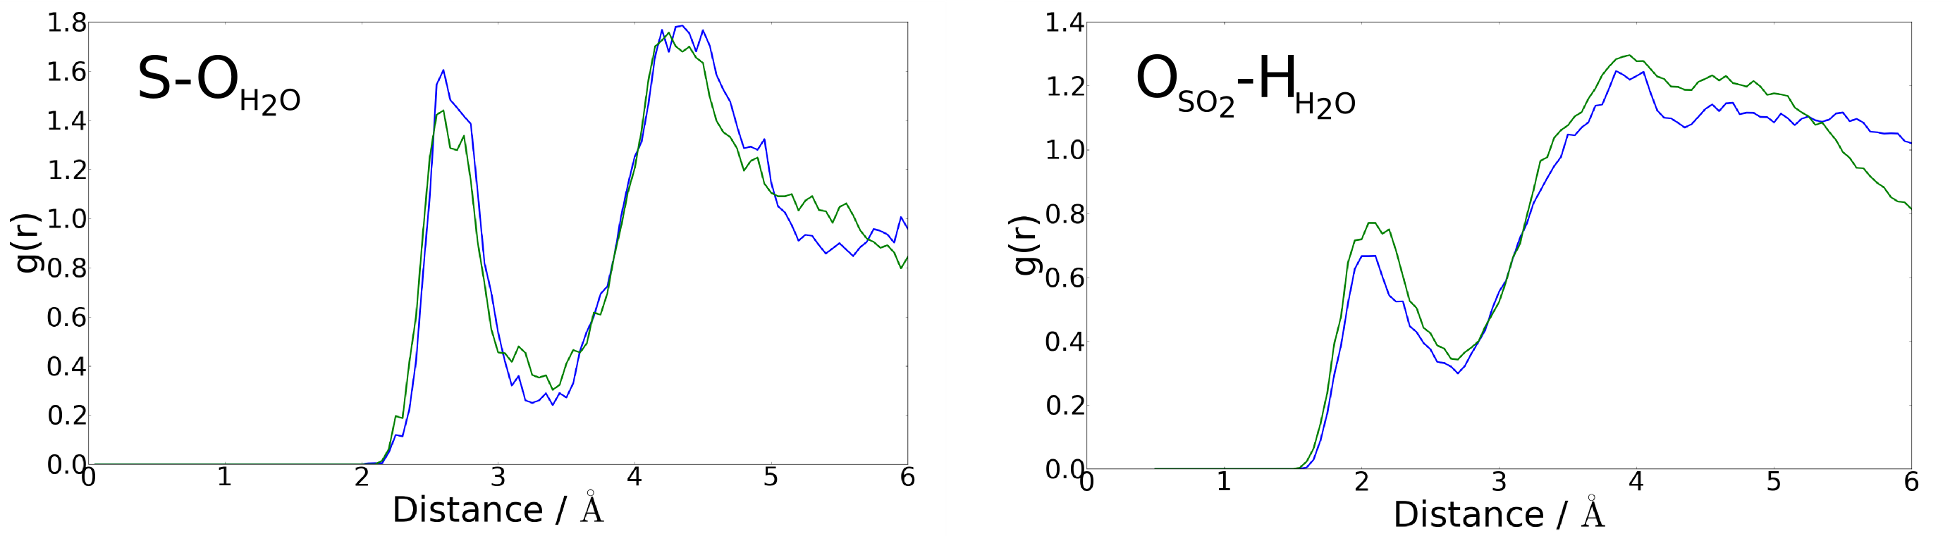
\includegraphics[scale=1.0]{images/rdf/rdf-small.png}
		\caption{Radial distribution functions (RDF) show the subtle change in how the hydrating waters around \suldiox~reposition as the temperature is increased from cold (blue) to hot (green). Shown are the two correlations between sulfur and water oxygens (left) and the \suldiox-oxygen and water hydrogens (right).}
		\label{fig:rdf}
	\end{center}
\end{figure}

\subsection {Bonding Transitions}

During the course of each simulation, the \suldiox~bonding coordination was determined and recorded for each timestep. From the coordination data we extract not only the populations of the various bonding coordinations, but also the frequencies of transitions between the different coordinations (i.e. the number of times each \suldiox~switched from one coordination type to another). With this data we have generated the directed graphs of Figure \ref{fig:coordination-transitions} depicting the cold and hot (Figure \ref{fig:coordination-transitions} A and B, respectively) bonding coordinations as circular colored nodes.\cite{Ellson2004,Gansner1999} The transitions between the coordinations are depicted as directed edges pointing in the direction of the transition from one coordination to another. The populations of the coordinations are depicted by both the node size and coloration (larger and darker red coordinations occur more frequently). Populations of the transitions between coordinations are depicted by arrow thickness, with thicker lines corresponding to more frequent transitions. Additionally, the transition lines are numbered to the right of each line with the number of times each transition occurred. 

\begin{figure}[h!]
	\begin{center}
		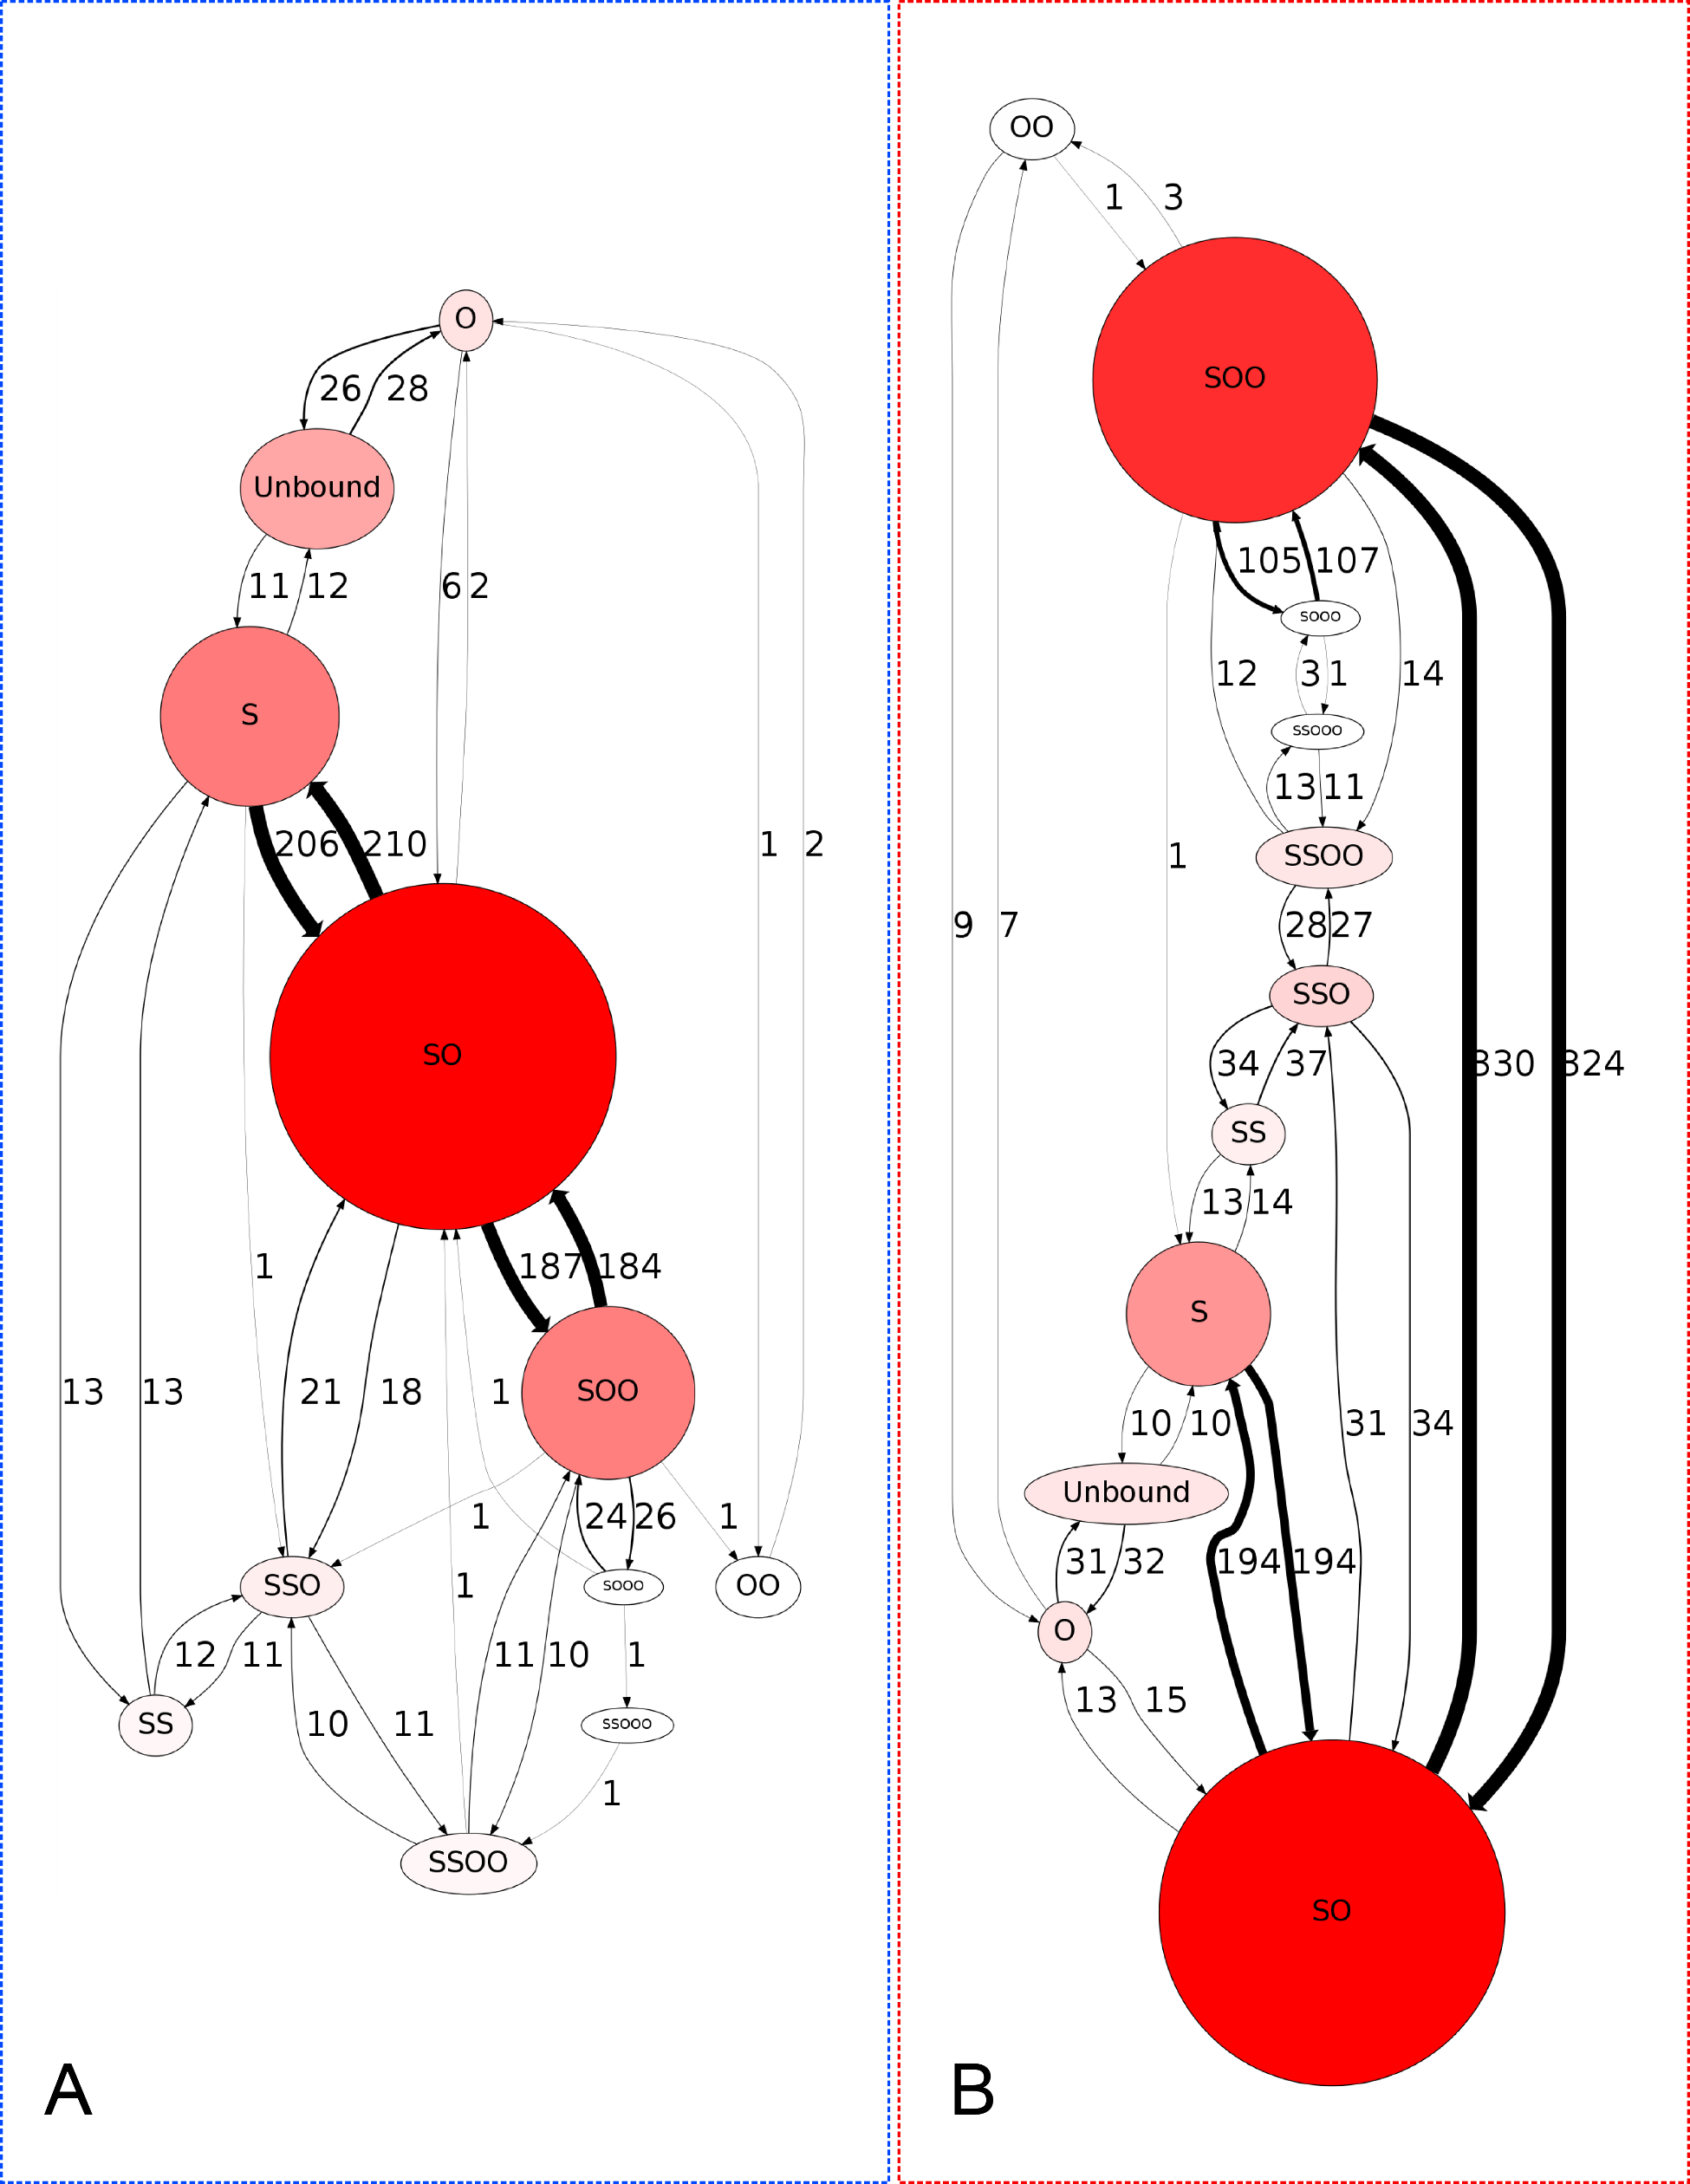
\includegraphics[scale=1.0]{images/coordinations/coordination-transitions.png}
		\caption{The bonding coordinations of \suldiox~on a water surface rapidly change as bonds break and form throughout the MD trajectories. Depicted here is a graph of the bonding coordinations, shown as colored nodes of varying size. Larger and more darkly colored coordination nodes are those more often encountered during MD (see Figure \ref{fig:bonding-coordinations}). The directed edges between the nodes represent the number of times the coordination transition occurred. Thicker lines correspond to a greater number of transitions between coordinations. The number of times a given transition occurred is labeled to the right of the corresponding line.}
		\label{fig:coordination-transitions}
	\end{center}
\end{figure}

As expected for the more populated coordinations, there are more transitions between larger nodes in Figure \ref{fig:coordination-transitions} than transitions to less populated coordinations. Insights to the bonding process are made clearer from these graphs. In the cold system graph of Figure \ref{fig:coordination-transitions}A, we find that the majority of transitions are between the ``S-SO'' and ``SO-SOO'' nodes. The number of transitions within this ``S-SO-SOO'' group of coordinations is an order of magnitude larger than any other transition. This indicates that while the \suldiox~is bound in any of the three most populated bonding coordinations, it is actively binding and unbinding the oxygens to form the other two coordinations in this group. Clearly, the \suldiox~is rather active and constantly forming and breaking bonds with its oxygens.

In the graph of the hot system in Figure \ref{fig:coordination-transitions}B, the transition frequencies follow the same trend as in the cold system, increasing with adjacent node size. One very surprising result is in the transition from ``SOO-SOOO''. This transition frequency does not follow from the adjacent node sizes, as the ``SOOO'' node represents less than 5\% of the bonding coordinations. This is indicative of a very rapid cycle of forming and breaking of bonds to the second \suldiox-oxygen. As noted earlier, it is likely that ``SOO'' coordinated \suldiox, asymmetrically binding twice through a single oxygen, is being pulled further into the water interface. It is likely more surrounded by waters, and in the hot system it can more easily form a brief third hydrogen bond to a water through the second \suldiox-oxygen. Because the triple-oxygen coordination is not as favorable, it quickly breaks the bond and the \suldiox~returns to the ``SOO'' coordination.

Given the information we have about the frequencies of bonding coordination transitions, it is possible to draw a likely route of adsorption beginning with an unbound \suldiox. From the unbound coordination, the \suldiox~can bind to waters either through the sulfur or an oxygen to enter the ``S'' or ``O'' coordinations, respectively. At both temperatures we find that the coordination transition in Figure \ref{fig:coordination-transitions} from unbound to ``O'' occurs almost three times more than the transition from unbound to ``S''. We find two possibilities that may explain this difference. The ``O'' coordination may form more easily, but also break quickly after formation, accounting for the higher transition frequency. Otherwise, the ``O'' coordination may be the first step in adsorption of an unbound \suldiox, where a subsequent addition of an \suldiox-sulfur interaction to a water oxygen would lead to a transition to the most frequent coordination, ``SO''. In the latter case, any adsorption of \suldiox~may proceed through an oxygen binding, accounting for the increased unbound-``O'' transition frequency.

To verify if the ``O'' coordination forms from, and breaks quickly to the unbound coordination as is suggested by the transition frequency plots in Figure \ref{fig:coordination-transitions}, we plot the lifespans of the various coordinations in Figure \ref{fig:coordination-lifespans}. Each point in the plot represents a time during the simulation in which the \suldiox~formed the respective coordination. The vertical ``lifespan'' position is calculated directly from the amount of time spent in the given coordination before changing to another. Both cold (blue) and hot (red) data are plotted. The data of Figure \ref{fig:coordination-lifespans} show that most coordination configurations last a very brief time, with the majority forming for under 0.5 ps. The three most populous coordinations, ``S'', ``SO'', ``SOO'' (as determined from Figure \ref{fig:bonding-coordinations} by percentage) in both temperatures have coordination lifetimes of up to 1 ps, in some instances lasting up to 1.5 ps. The brevity of lifespans overall speaks to the dynamic nature of the interface. The length of time in each coordination parallels the populations of the coordinations, and suggests an ordering of steady states among various bonding coordinations. The ``unbound'' configuration stands out as an anomaly amongst the lifespans of the other bonding coordinations. The few lifespans above 1.5 ps, up to 3.25 ps long, suggest a \suldiox~that not only unbinds from the water surface, but that it also recedes far enough to avoid a quick rebinding and coordination change to ``S'' or ``O''. Those few long lived unbound data points indicate times when the \suldiox~is far from the water, residing in the gas phase until the necessary water rearrangement occurs and it is drawn back to the surface to rebind.

\begin{figure}[h!]
	\begin{center}
		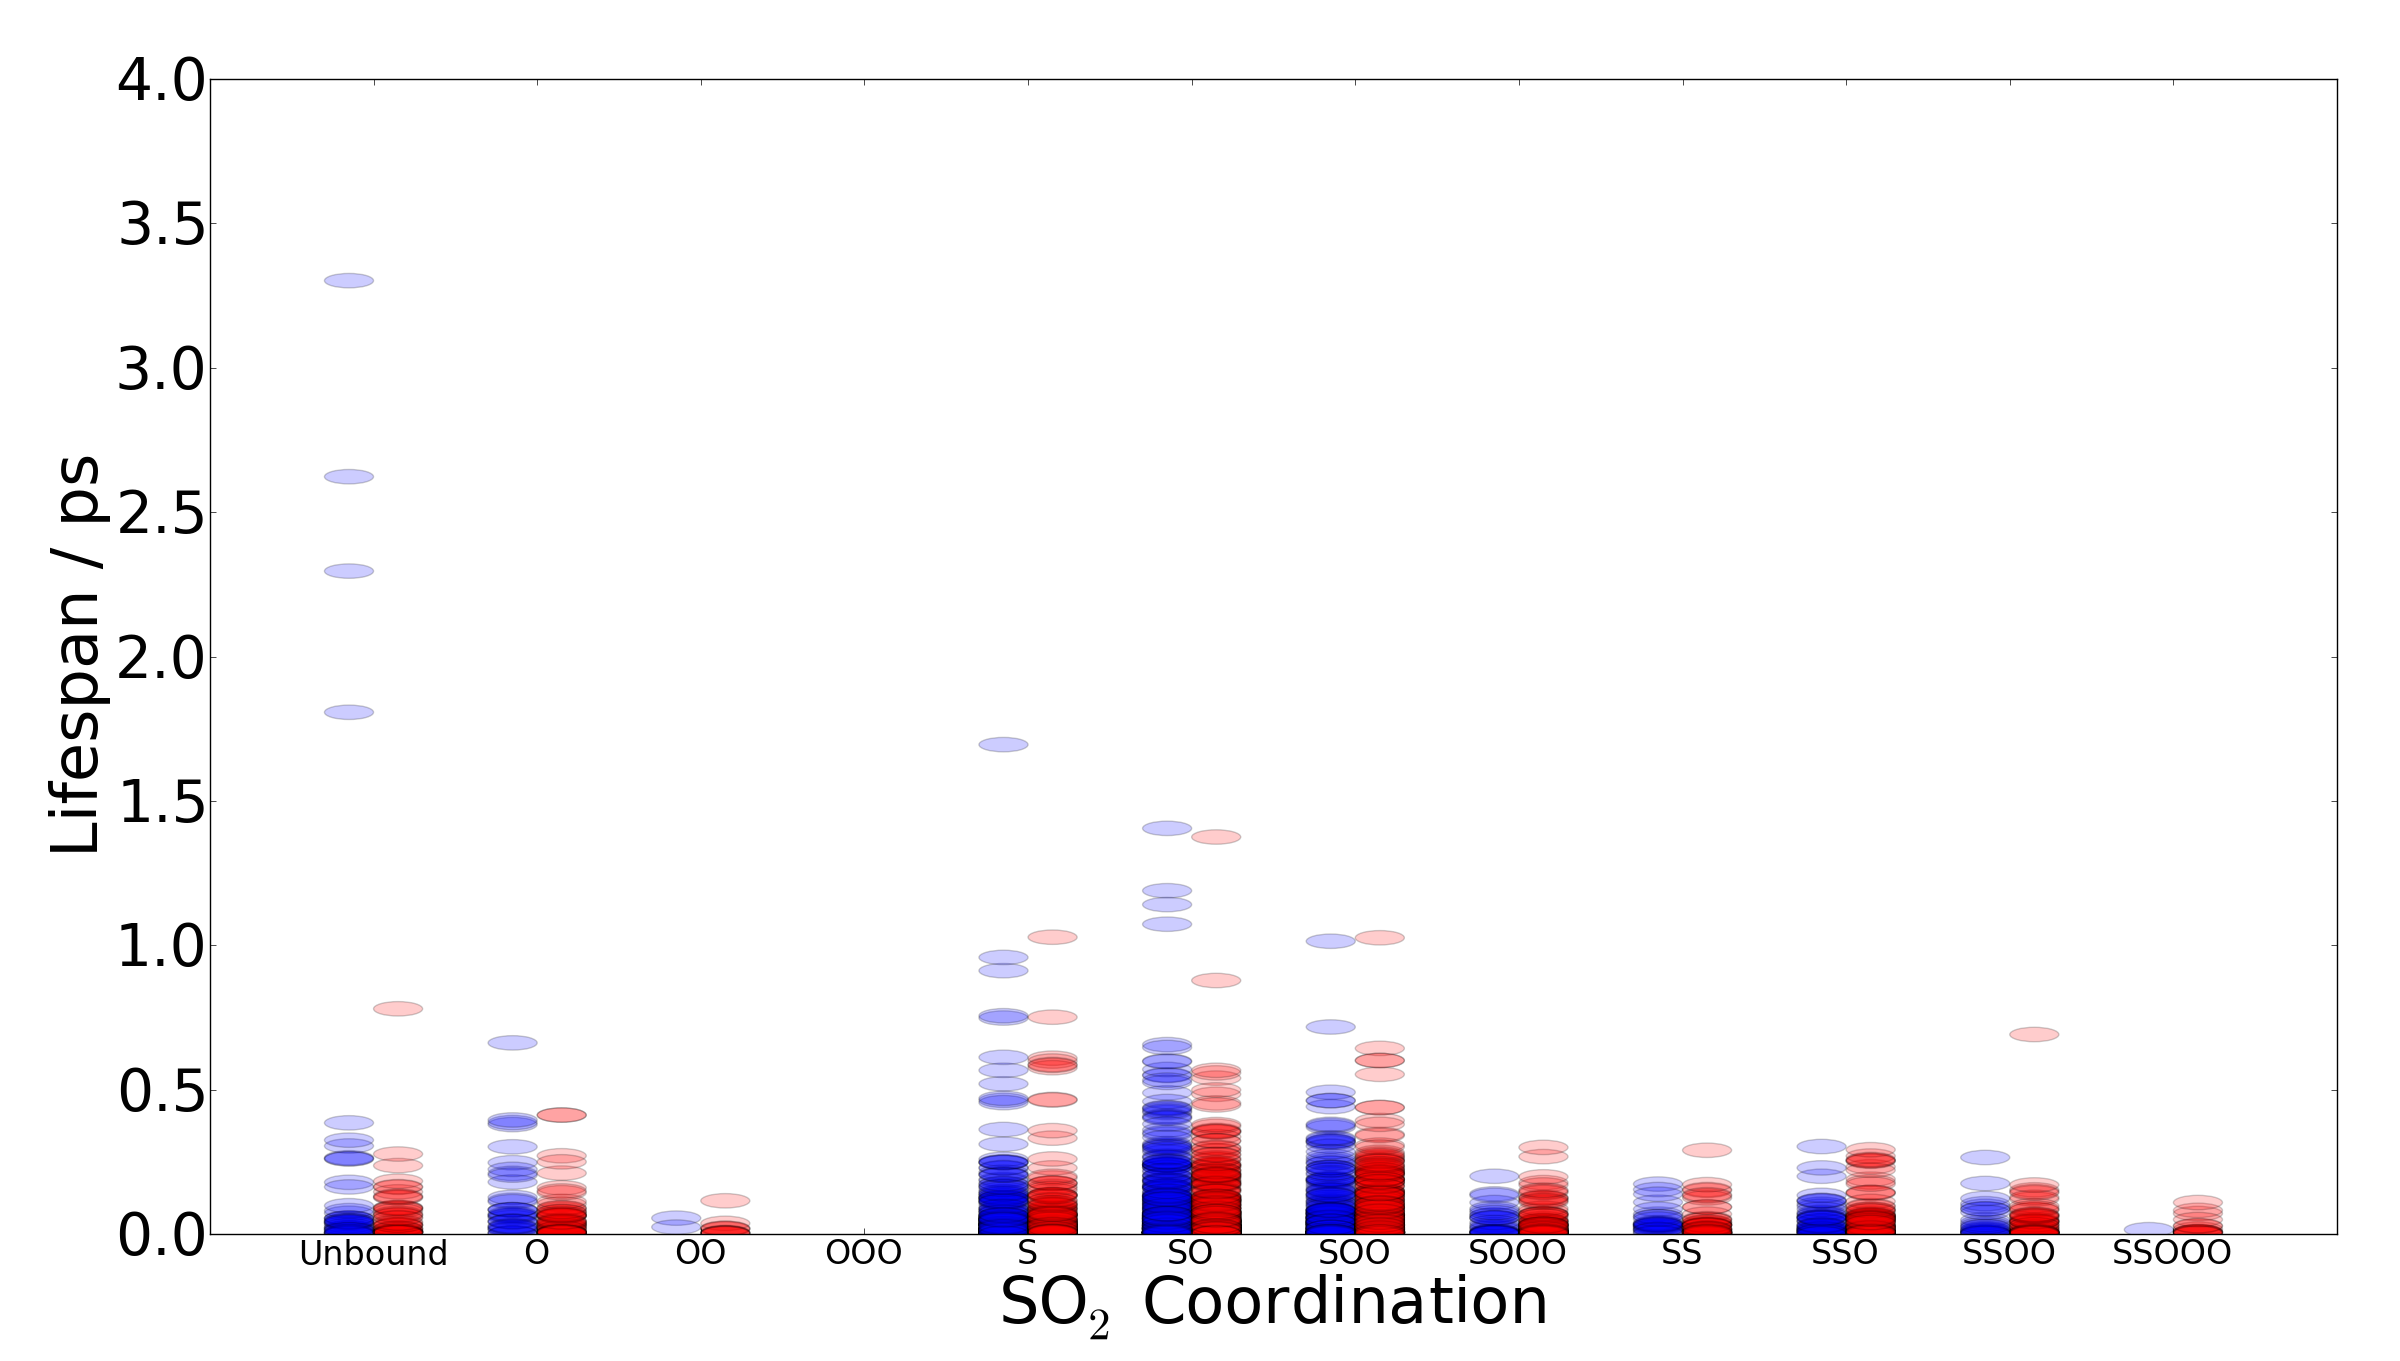
\includegraphics[scale=1.0]{images/coordinations/coordination-lifespans.png}
		\caption{Given that certain bonding coordinations of the surface \suldiox~are more often encountered than others (see Figure \ref{fig:bonding-coordinations}), the plot here shows the time spent in each bonding coordination. Each point in the plot represents a single span of simulation time that the \suldiox~had the given coordination. The total amount of consecutive timesteps in a coordination corresponds to the vertical position along the lifespan axis, in ps.}
		\label{fig:coordination-lifespans}
	\end{center}
\end{figure}

Returning to the transition plots of Figure \ref{fig:coordination-transitions}, the behavior of the unbound transition to both ``S'' and ``O'' coordination can now be better characterized. Figure \ref{fig:coordination-lifespans} shows that the ``O'' coordinated lifetimes are shorter than the ``S'' coordinated ones. Figure \ref{fig:coordination-transitions} shows that the unbound-``O'' transition occurs almost three times more than the transition to the ``S''. The unbound \suldiox~forms a bond to a neighboring water through its oxygen, but that bond is short-lived and either quickly breaks (resulting in unbound \suldiox), or it transitions to the ``SO'' coordination by forming another bond through the sulfur. The unbound-``S'' transition does not occur as often. This may be because the ``S'' coordination is more stable than the ``O''. Once in the ``S'' coordination the \suldiox~does not quickly break the interaction from its sulfur to water, but rather remains for up to 1 ps in the ``S'' coordination before (most likely) forming an oxygen bond to make the ``SO'' coordination. We have outlined the likely behavior of \suldiox~as it transitions from the gas phase in an unbound coordination to binding to an aqueous interface by forming bonds and interactions with surface waters.

Once the \suldiox~begins interacting with the water surface, the pathway leading back to the unbound coordination is not often traversed. As shown in Figure \ref{fig:coordination-transitions} the dominant coordination transitions occur between the ``S-SO-SOO'' group of coordinations. This suggests that the \suldiox-sulfur interaction to a water oxygen has a much longer lifespan than the oxygen bonding to water hydrogens. The difference between the ``S-SO-SOO'' coordinations is an addition or removal of oxygen bonds, and the frequent transitions between them show that the bonds to \suldiox-oxygens are quickly forming and breaking. For the \suldiox-sulfur interaction to break, the \suldiox~must enter a non-sulfur coordination (e.g. ``O'', ``OO'', unbound, etc.) or a coordination with more than a single sulfur interaction (e.g. ``SS'', ``SSO'', etc.). The transitions to coordinations that allow for breaking of the \suldiox-sulfur interactions, or switching the interaction to another water, are infrequent compared to those leading to an oxygen bond transition. Thus, the \suldiox~spends most of its time while bound to the surface waters breaking and forming hydrogen-bonds through its oxygens, and interacting with neighboring waters through a more persistent interaction via the \suldiox-sulfur atom.

\subsection{Cyclic \suldiox~Hydrate Structures}

Having examined the bonding coordinations and bonding behavior of \suldiox~with surface waters, we now turn to a secondary behavior of the hydrate structures that form around the surface-bound \suldiox~molecule. The simulation trajectory data was analyzed to determine the presence and characteristics of \suldiox~cyclic hydrate structures that form during MD, as posited earlier and depicted in Figure \ref{fig:cyclic-structures}. Only the most commonly occurring subset of the cyclic structures were analyzed. 

\begin{figure}[h!]
	\begin{center}
		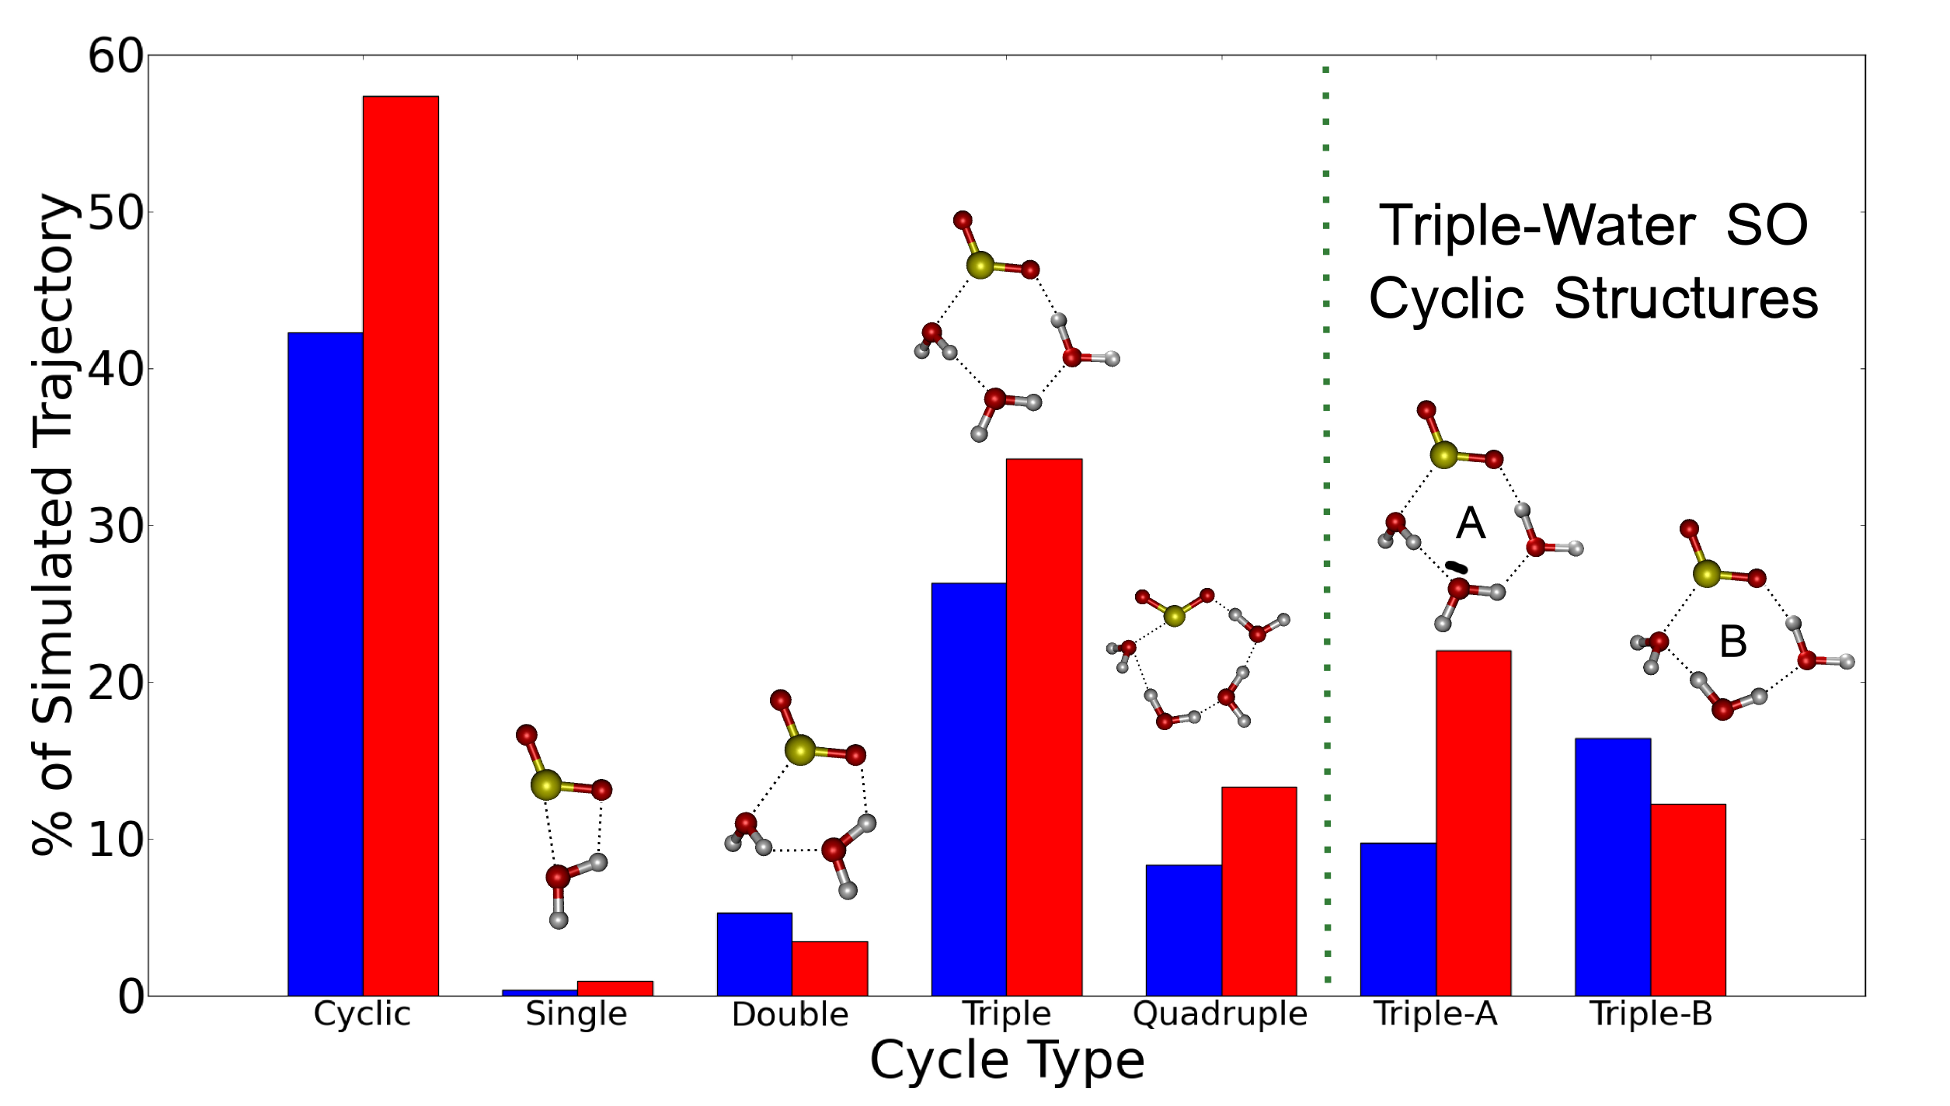
\includegraphics[scale=1.0]{images/cycles/SO-cycle-breakdown-with-cartoons-small.png}
		\caption{}
		\label{fig:cyclic-breakdown}
	\end{center}
\end{figure}
The plot in Figure \ref{fig:cycle-breakdown} shows the distribution of how often the various types of cyclic hydrates were encountered at both cold (blue) and hot (red) temperatures. Each data point shows a percentage of the MD trajectories in which the \suldiox~was a member of a cyclic structure, for different numbers of cyclic waters (up to 4). The two tallest data points, left-most in the plot, show the overall time spent in all types of cyclic structures. Clearly the hot system \suldiox~spends more time in a cyclic structure than at the cold temperature. The plot is based on two criteria for determining if a cyclic structure has formed. (1) The distances between atoms must match the same bonding/distance criteria as used for determining bonding coordinations. (2) The \suldiox~must be minimally in a bonding coordination of type ``SO'', meaning that the sulfur has at least one bonding interaction, and at least one hydrogen-bond must have formed with an oxygen to a neighboring water-hydrogen. As noted earlier in the discussion of the graph-finding routine and the BFS algorithm, the cyclic structures found represent the smallest cycles in which the \suldiox~is a member, based on order of discovery. The \suldiox~will be inevitably involved in other larger and more extended cyclic bonding structures beyond the first one discovered via the BFS. The larger and more extended cyclic structures involving more waters affect the behavior of the hydrogen-bonding network of the water surface. However, we focus here only on the smallest cycles involving the \suldiox~as the most affect the \suldiox~bonding and hydrating behaviors.

It is remarkable that the difference of the time spent in a cyclic structure between the two temperatures is 15\% (42\% cold, 57\%hot). The hot \suldiox~spends well over half of the simulated time bound as one of the hydrate cycles, and the cold \suldiox~spends just under half of the time as such. Thus, in addition to having found the most likely bonding coordination during the simulated life of \suldiox, we have also found that the hydrates of the \suldiox~form a cyclic structure for much of the time it is bound to the water surface.

Now we look at the different types of cyclic hydrates, distinguished by the number of waters involved in the bonding structure. In Figure \ref{fig:cyclic-breakdown} the single and double water cycles are the least frequently encountered structures, accounting for less than 10\% of both temperature simulations. Formation of the single type is likely energetically unfavorable because of the proximity of the single water to the \suldiox. The double-water structure was one of two types of clusters proposed in a previous computational work as a candidate structure contributing to the overall IR spectrum of surface-bound \suldiox.\cite{Baer2010} In the static and geometry-optimized cluster calculations, lacking the extended water structure or bonding from waters external to the hydrate, both the double and triple types appear equally likely to form. However, the MD simulations here have introduced many waters into a dynamic environment allowing for extended bonding networks, and the results show clearly that the double-water cyclic hydrate is formed much less often (less than 5\% at both temperatures) than the triple-water form.

The results for triple and quadruple-water structures show that larger hydrate cycles are favored at higher temperatures. Although the higher number of hydrating waters (>4) are not shown, those contribute minimally to the overall distribution. The majority of the cyclic hydrates are formed with three waters in the triple type. This hydrate type matches the bonding structure inferred from our previous experiments, and also one of the cluster types modeled by others.\cite{Tarbuck2005,Tarbuck2006,Baer2010} It was further found that of the triple-type hydrate cycles, the waters contributing to the cycles can be arranged in two ways that preserve the hydrogen-bonding between the molecules. The two triple cycle structure are depicted on the right side of Figure \ref{fig:cyclic-breakdown}, along with the plots of the contributions to the overall distribution. It is notable that each temperature has a different dominant type of triple-water cyclic structure. The cold system forms more of the type-B, and the hotter system forms primarily triple type-A.

\subsection {Cyclic Structure Energy Calculations}

\subsection {Cyclic Hydrate Structure Lifetimes}

Knowing that the \suldiox~bound to a water surface is most likely in the ``SO'' bonding coordination, and also often taking part in some type of cyclic structure, how long does the cyclic hydrate form before breaking to an acyclic structure? To answer the questions of cyclic lifespans, a method was devised to define a lifetime of a cycle. For each trajectory, the coordinate data was analyzed to determine if a cyclic hydrate structure was formed based on the bonding distance criteria established earlier in this manuscript. A timeline was then produced where each timestep was given a value of 1 or 0 if a \suldiox~cycle was found or not found, respectively. This resulted in a time-function, $C(t)$, similar in nature to a digital signal. The resulting cycle formation time-function is plotted for one of the simulated trajectories shown as the dashed black line in Figure \ref{fig:debouncing}. At the far left of the plot the function is in the ``no cycle'' state, and then switches ``on'' as a cycle is formed. The cyclic structure is very dynamic constantly moving and distorting, so any of the bonds forming the cyclic bonding structure are liable to break and reform quickly. This is manifested in Figure \ref{fig:debouncing} as a series of very sharp spikes in the function lasting less than 10 fs each. Because of the very rapid breaking and reformation of the cyclic structure, a procedure was used to ``debounce'' the time-function to disregard very brief moments when the cycle breaks or forms for less than 20 fs. The time-function, $C(t)$ was smoothed using a moving gaussian window function with a 10 fs width. The resulting smoothed function, $C_s(t)$, was then cutoff with the following criteria:

\[
  f(t) = \left\{ 
  \begin{array}{l l}
    0 & \quad C_s(t) < 0.2\\
    1 & \quad C_s(t) \geq 0.2\\
  \end{array} \right.
\]

where $f(t)$ is the debounced time-function that better represents the lifespans of cycles, eliminating the very brief discontinuities and excursions outside the bonding criteria that cause the rapid ``bouncing'' of the cyclic time-function, $C(t)$. Figure \ref{fig:debouncing} shows the original time-function of cycle formation and breaking, $C(t)$ (dashed black), the smoothed function, $C_s(t)$ (red), and the final ``debounced'' function, $f(t)$ (green).

\begin{figure}[h!]
	\begin{center}
		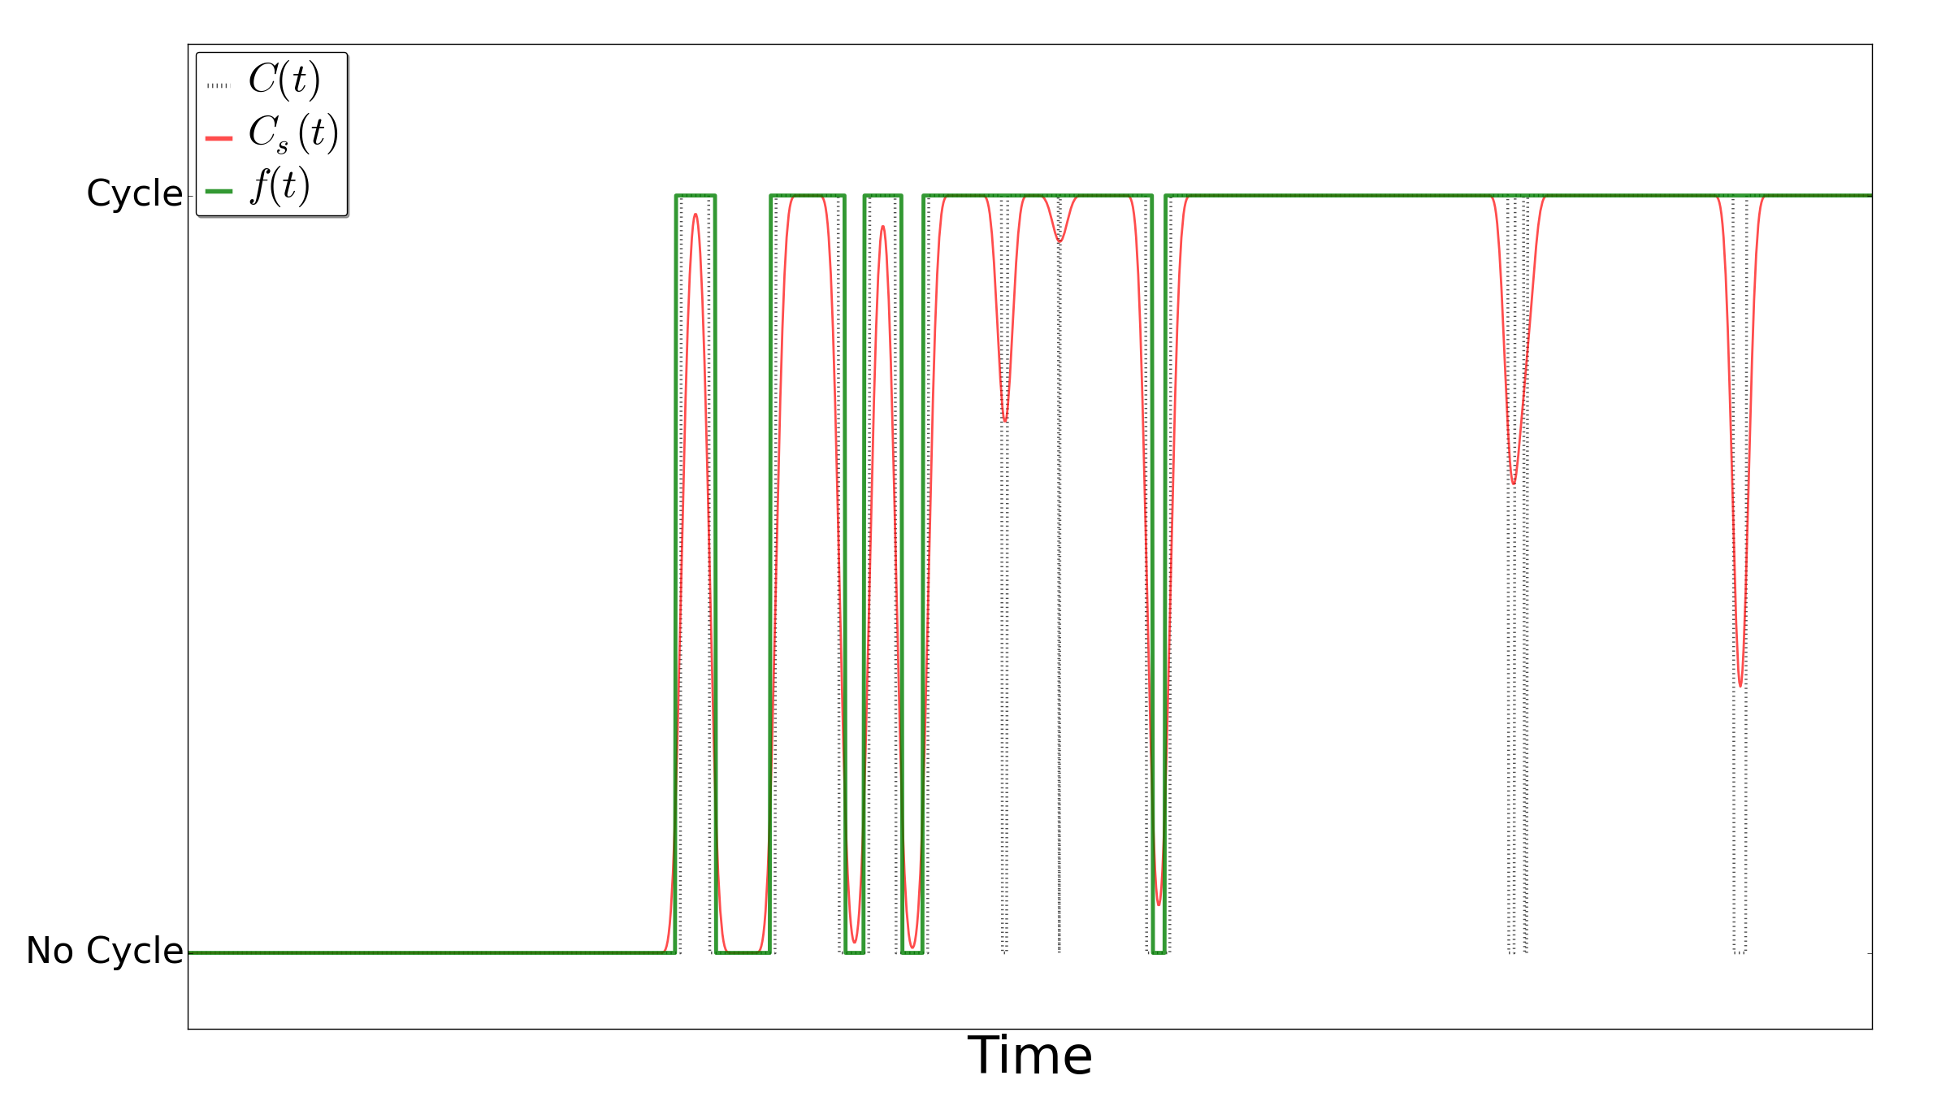
\includegraphics[scale=1.0]{images/cycles/cycle-debouncing-small.png}
		\caption{}
		\label{fig:debouncing}
	\end{center}
\end{figure}

The distribution of cycle lifetimes (i.e. contiguous spans of time spent with $f(t) = 1$) was determined. A plot of the cyclic lifespans is shown in Figure \ref{fig:cycle-lifespans} for the cold (blue) and hot (red) simulations. The most frequent lifespan for both temperature data sets lasts between 0-1 ps. This accounts for the vast majority of cyclic hydrates found (approximately 95\%) indicating that these structures are very transient, and are continuously forming and breaking for very short periods of time. Even with the ``debouncing'' procedure that would artificially increase the timespan spent either formed or broken, the nature of the water surface, and the very dynamic extended hydrogen bonding network, keeps many of the structures from lasting much longer than 1 ps. The difference between hot and cold systems in the $<1$ ps population is less than 2\%, with this trend also extending to the longer lifespans as well. The inset of figure \ref{fig:cycle-lifespans} shows an expanded view of the region above 1 ps. All of the distribution shows only a $<1.5$\% difference between cold and hot cyclic lifetimes. Overall, the distribution shows that when cycles form, at both temperatures, they last a similar amount of time. 

Up to 3 ps, the cold temperature cycles show a very slight population increase above the hot temperature cycles. Above 4 ps, most of the cycles that form are found in the hot system. The 8 ps cycles are notable in that they form  for just under half of an entire single simulated trajectory.

We know from the transition frequency plots of Figure \ref{fig:coordination-transitions} that the bonding coordinations are switching frequently. The \suldiox~is likely forming and breaking bonds with waters extraneous to the cyclic hydrate structures (i.e. not directly involved in the bonds of the cycle). For the longer-lived cycles, the extraneous bonding to the \suldiox~may have little effect on the cyclic hydrate waters. However, any time the \suldiox~switches into an unbound, sulfur-only, or oxygen-only coordination (i.e. ``S'', ``SS'', ``O'', etc), the cyclic structure is necessarily broken. Because the majority of cyclic structures last only briefly ($<1$ ps), the active switching of \suldiox~bonding coordinations appears to break the cyclic structure. Figure \ref{fig:bonding-coordinations} shows the sum of coordinations that necessarily break cyclic structures account for approximately 39\% and 24\% of the bonding coordinations in the cold and hot system, respectively. Consequently, the distribution of Figure \ref{fig:cyclic-breakdown} also indicates that there are more cycles formed in the hot system (approximately 16\% above the cold). The increased temperature appears to cause the \suldiox~to bond in such a way that is more conducive to the formation of cyclic structures. Furthermore, the distribution of bonding coordinations in the hot system shifts the transition between bonding coordinations away from cycle-breaking coordinations (i.e. those coordinations that necessarily disallow cycle formation). This possibly accounts for the slightly increased populations of longer cycle lifespans in the hot system (greater than 4 ps in some cases) compared to the cold system in the cycle lifespan distribution of Figure \ref{fig:cycle-lifespans}. 

\begin{figure}[h!]
	\begin{center}
		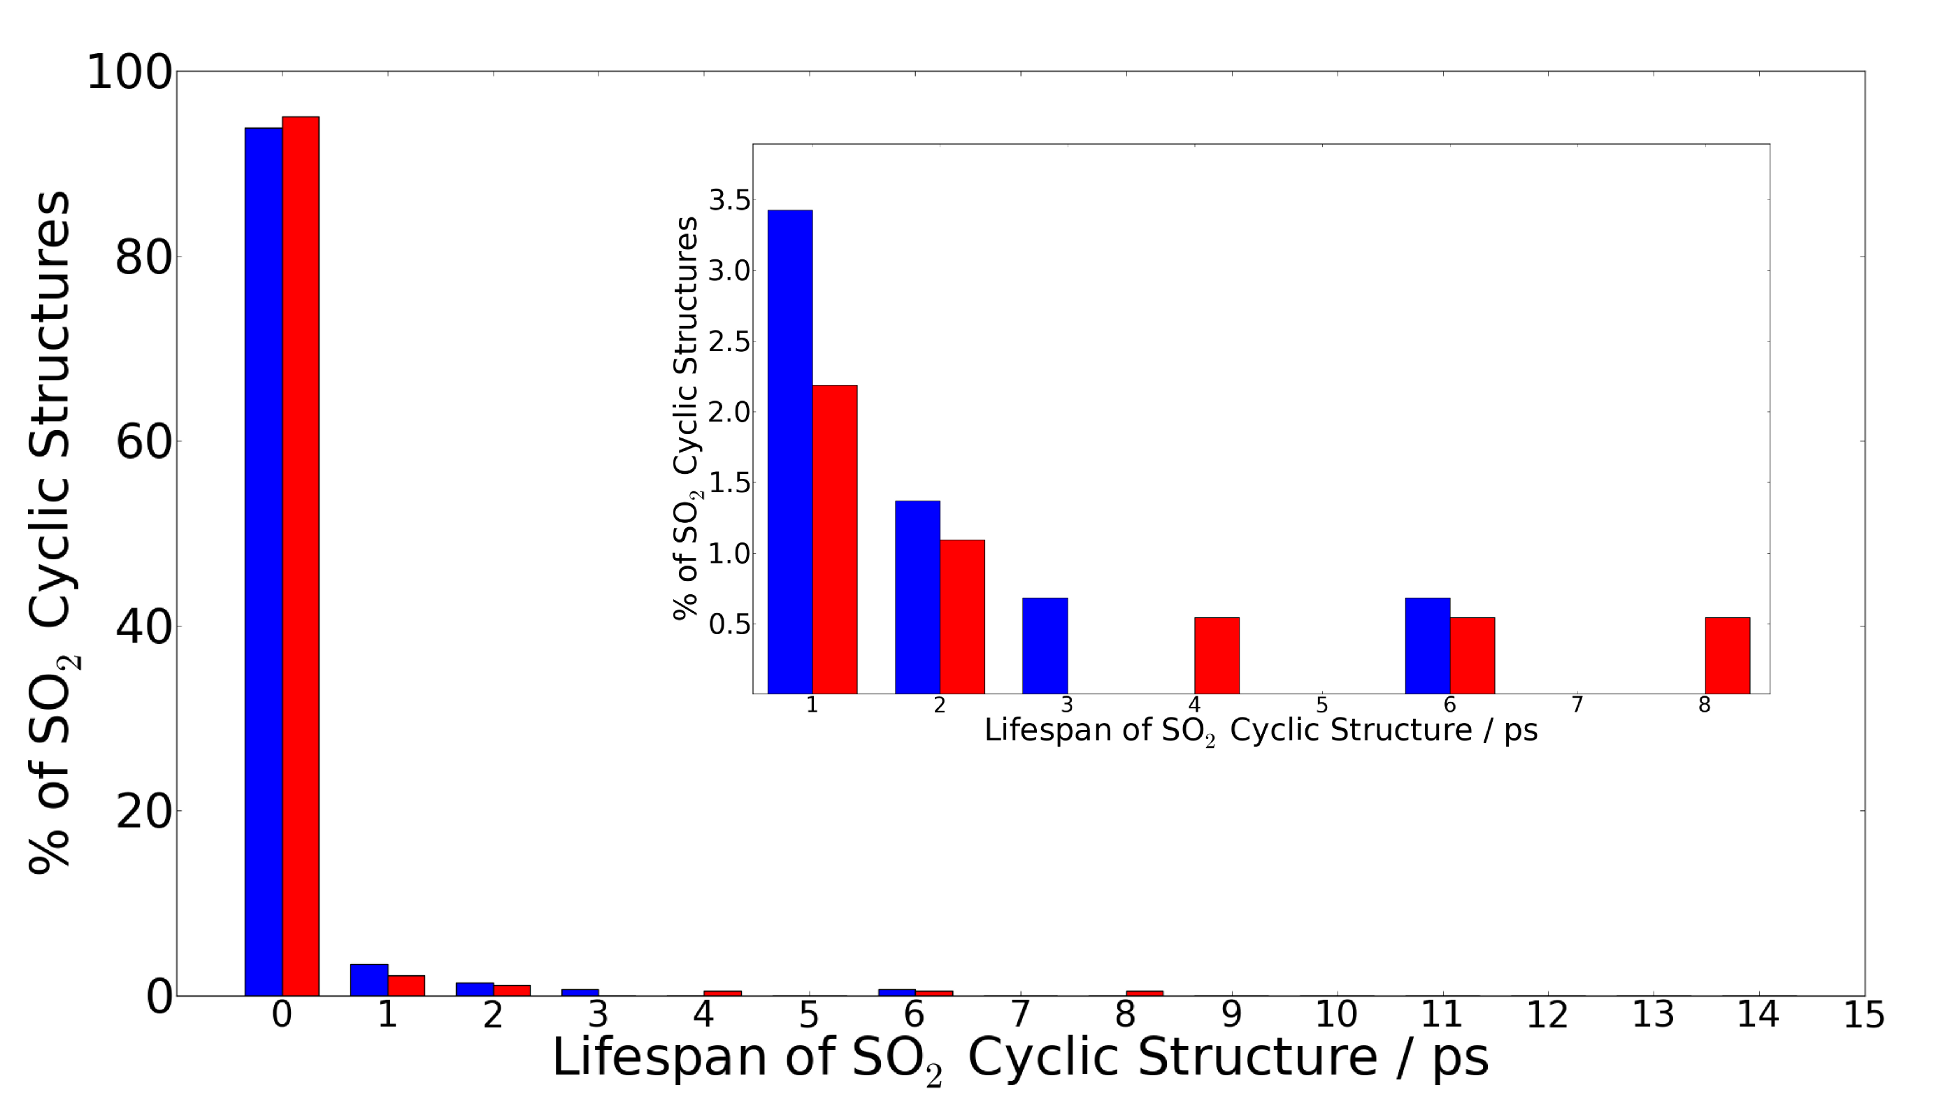
\includegraphics[scale=1.0]{images/cycles/cyclic-lifespans-inset-small.png}
		\caption{}
		\label{fig:cycle-lifespans}
	\end{center}
\end{figure}

\section {Conclusions}

The adsorption of small gas molecules to water surfaces has been extensively studied over the past few decades. Much has been learned about the energies of hydrate configurations, and the kinetics of gaseous uptake into aqueous systems. Yet, the specific nature of the adsorption process, including the various geometries, hydrate species, and bonding pathways remains largely unknown. As a gas transitions into the liquid water phase, it passes through a fluid interfacial region that remains poorly understood. Our understanding of the processes and chemistry of the interface is still in its infancy, but we gain unique new insights that are key to understanding many environmentally important processes at aqueous surfaces.

Presented herein are the results of ab initio molecular dynamics simulations that focus on how a wandering gaseous \suldiox~molecule first makes contact with a water surface, and subsequently forms extended hydrate structures with interfacial water molecules. The computational studies complement and expand on experimental studies from this laboratory that found surface complexation of \suldiox~at a water surface.\cite{Tarbuck2005,Tarbuck2006,Ota2011} Furthermore, these computations build upon and enrich our understanding of adsorbing \suldiox~behavior from our recently published computational study on interfacial geometries of aqueous surface \suldiox~molecules.\cite{Shamay2011}

Our simulations show that \suldiox~has a preferred means of bonding and interacting with surface water molecules by taking on various bonding coordinations. In this work it was shown that the ``SO'' bonding configuration is the most preferred, with ``S'' and ``SOO'' also contributing greatly to the coordination distribution. Once a \suldiox~has bound to form a surface hydrate it rarely forms multiple bonding interactions through the sulfur atom, and even less frequently takes on a configuration with no sulfur interactions to nearby waters.

This study is one of very few temperature studies looking at the microscopic nature of interfacial gas molecules on water. By changing the temperature, it was found that a hotter water system leads to longer \suldiox~binding to the water surface. The distribution of bonding coordinations was greatly affected by a temperature change, shifting populations of bonding configurations because of the altered \suldiox~and \wat~behavior. At the higher temperature, \suldiox~forms more frequent bonds to interfacial waters through the sulfur and oxygen atoms. Overall, we have determined that the \suldiox~hydrate interactions are transient, binding and unbinding to water molecules rapidly in very dynamic bonding coordinations.

In this work we introduce the use of a graph structure to represent atoms and interconnectedness between molecules, and also to represent transitions between the various bonding coordinations of an adsorbed \suldiox. It was shown that the intermolecular bonds formed through the \suldiox-oxygens are quickly broken and formed, lasting briefly compared to sulfur interactions. From the graph of bonding coordination transitions, we found a likely pathway for \suldiox adsorption starting with an unbound gas-phase \suldiox, ending with a hydrated \suldiox~species bound to surface waters.

The formation of cyclic hydrate structures was probed and it was found that these hydrated bonding ring species form during much of a simulated trajectory. Temperature increases the occurrence of cyclic structures, and also shifts the distribution of the specific types of cycles being formed. Two types of cyclic tri-hydrates were discovered during the course of simulations. The cycle lifetimes were found to be mostly short-lived, with a majority lasting less than 1 ps before breaking and reforming due to the dynamic bonding and motion of the surface waters and \suldiox~molecules. Temperature did not have a very dramatic effect on the cyclic lifespans, but higher temperatures did lead to \suldiox~bonding coordinations that are more likely to form into cyclic hydrates.

These studies build upon our computational and experimental research in this area, seeking to understand how gases adsorb and transit across an aqueous/air interface. Such knowledge is invaluable for understanding land water and environmental aerosol systems where gaseous uptake behavior at a water surface surprises us and often defies our physical intuitions.\cite{Jayne1990,Yang2002,Worsnop1989,Boniface2000}


\bibliography{bib/so2temperature}

\end{document}
